\documentclass[12pt]{report}
\usepackage[a4paper,width=150mm,top=25mm,bottom=25mm,bindingoffset=6mm, includefoot, includehead]{geometry}

\usepackage[utf8]{inputenc}
\usepackage[italian]{babel}
\usepackage{alphabeta}
\usepackage{biblatex}


\usepackage{array} % per tabelle
\usepackage[table]{xcolor}
\usepackage{multirow}
\usepackage{longtable}
\usepackage{changepage}
\usepackage[export]{adjustbox}

\usepackage{amsfonts}
\usepackage{amsmath}
\usepackage{amssymb,amsmath,color}
\usepackage{graphicx}
\usepackage{float}
\usepackage{standalone}
\usepackage{changepage}
\usepackage{wrapfig}

\usepackage{graphicx}
\usepackage{fancyhdr}
\usepackage{float}
\usepackage{color}
\usepackage[nottoc]{tocbibind}
\usepackage{xcolor}
\usepackage{titlesec}
\usepackage{amssymb}
\usepackage{multicol}

\usepackage{pdfpages}

\usepackage{placeins} %for floatBarrier

\addtolength{\skip\footins}{2pc plus 5pt}

\setlength{\arrayrulewidth}{0.5mm}
\setlength{\tabcolsep}{10pt}
\renewcommand{\arraystretch}{1.6}
\setlength{\parindent}{0cm}%no indent

% Definizione colori
\definecolor{opal}{rgb}{0.66,0.76,0.74}
\definecolor{uclablue}{rgb}{0.33, 0.41, 0.58}

\usepackage{hyperref}

\hypersetup{
    citecolor=black,
    colorlinks=true,
    linkcolor=black,
    filecolor=magenta,      
    urlcolor=black,
    pdftitle={Progetto Sistemi Digitali}
    }
    
\usepackage{minted}
\usemintedstyle{manni}

\newcommand\myemptypage{
    \null
    \thispagestyle{empty}
    \newpage
}


\usepackage{pgfplots}


\usepackage{fancyhdr}
% Stile di pagina
\pagestyle{fancy}
\definecolor{LightGray}{gray}{0.9}
%\usemintedstyle{manni}

\bibliography{documentazione} % put your bibliography here

\raggedbottom

\graphicspath{{figs/}}

\begin{document}
	


%%%%%% First Page %%%

\pagestyle{myheadings}


\thispagestyle{empty}  
                                               
\begin{center}                                                            
    \vspace{2mm}
    {\large ALMA MATER STUDIORUM -- UNIVERSIT\`A DI BOLOGNA} \\  
                         
      \vspace{2mm}
\end{center}
\begin{center}



\end{center}
\begin{center}
      \vspace{5mm}
      {\large \uppercase{Scuola di Ingegneria e architettura}} \\
        \vspace{5mm}
       {\large Dipartimento di Informatica - Scienza e Ingegneria}\\
   		{\large DISI}\\
        \vspace{5mm}
      {\Large \bf Corso di Laurea magistrale in ingegneria informatica}\\
      \vspace{15mm}
      { \large\textbf{Progetto}\\ di\\ \textit{Sistemi Digitali M}}\\
      \vspace{5mm}
      {\LARGE\bf Stalker-bot} \\                
      \vspace{20mm}
\end{center}

\par
\noindent
\begin{minipage}[t]{0.47\textwidth}
{\large{\bf Professori:\\
Prof. Stefano Mattoccia\\ Prof. Matteo Poggi}}
\end{minipage}
\hfill
\begin{minipage}[t]{0.47\textwidth}\raggedleft
{\large{\bf Autori:\\
Davide Di Molfetta\\
Lorenzo Venerandi\\}}
\end{minipage}
\vspace{20mm}
\begin{center}
{\large{\bf Anno Accademico 2022-2023}}
\end{center}


\vfill

%%%%%% ABSTRACT %%%%%%%%%%\clearpage
\clearpage
\null
\thispagestyle{empty}
\clearpage

\chapter*{Abstract}
Stalker-bot \`e un piccolo robot mobile, cingolato, controllato da un Raspberry Pi 4B che comunica con un Arduino Nano. Il suo compito \`e quello di unire la potenza del riconoscimento facciale all'efficacia dei dispositivi embedded. Grazie ad una camera e ad una prima fase di addestramento in cui Stalker-bot impara a riconoscere una specifica persona (proprietario), egli \`e in grado di individuare la posizione del volto e di seguirne i movimenti.

%%%%%% INDEX %%%%%%%%%%
\tableofcontents
\thispagestyle{empty}

 

%%%%%%% BODY %%%%%%%%%
\clearpage
\null
\thispagestyle{empty}
\clearpage

\pagestyle{plain}
\chapter*{Introduzione}
\addcontentsline{toc}{chapter}{Introduzione}

\section*{Motivazioni}
\addcontentsline{toc}{section}{Motivazioni}
Le motivazioni dietro la realizzazione di "Stalker-bot" sono principalmente legate alla volont\`a di acquisire conoscenze e competenze per l'integrazione tra pi\`u sistemi embedded e principi di machine learning e computer vision. Per poter affrontare questo progetto \`e stato necessario acquisire una maggiore dimestichezza nell'utilizzo di strumenti software e hardware coinvolti. Nello specifico, OpenCV si \`e rivelato fondamentale per la realizzazione in prima battuta dell'addestramento e in secondo luogo del riconoscimento facciale .
	
\section*{Riconoscimento facciale}
\addcontentsline{toc}{section}{Riconoscimento facciale}
Il riconoscimento facciale \`e una tecnica molto diffusa al giorno d'oggi che permette di individuare e riconoscere volti umani.
Questa tecnica sottintende la capacit\`a di individuare la presenza e la posizione di determinati oggetti all'interno di un'immagine o di un video. Questa sotto-capacit\`a \`e conosciuta anche come "object-detection".
Grazie all'object detection, spesso viene segnalata la posizione dell'oggetto, all'interno dell'immagine o del video, tramite una bounding box, ovvero un rettangolo che circonda l'oggetto.



\section*{Contenuti}
\addcontentsline{toc}{section}{Contenuti}
Questo progetto descrive il flusso di lavoro per lo sviluppo di un piccolo robot mobile in grado, mediante una camera e uno stream video fornito da essa, di: imparare come \`e fatto il volto del suo proprietario (anche pi\`u di uno), riconoscere quest'ultimo e seguire i movimenti del suo volto. In prima battuta \`e
stato necessario scegliere i sistemi embedded pi\`u opportuni; in secondo luogo sono stati selezionati tutti i componenti elettronici da coinvolgere; successivamente \`e stato sviluppato il software per addestrare il robot a riconoscere il suo proprietario e per riconoscimento durante uno flusso video; infine, dopo aver effettuato una serie di test soddisfacenti, ci si \`e occupati di creare la struttura fisica che dovesse contenere il tutto: la scelta è ricaduta sulla stampa 3D.

	
\section*{Organizzazione}
\addcontentsline{toc}{section}{Organizzazione}
Nel primo capitolo viene riportata una descrizione della libreria utilizzata per la realizzazione dell'addestramento e del riconoscimento facciale.
Nel secondo capitolo, invece, viene prima fornita una panoramica su tutti i componenti utilizzati per la realizzazione di questo progetto, e successivamente viene riportata una descrizione pi\`u dettagliata dei principali componenti.
Nel terzo capitolo viene prima descritta la struttura del robot, in particolare vengono mostrati i collegamenti tra i vari componenti elettronici e sono riportati i vari elementi che compongono la scocca del robot. In fondo a questo capitolo viene anche mostrato come \`e stato assemblato il tutto.
Nel quarto capitolo viene riportato e commentato come \`e stato realizzato lato software l'addestramento, il riconoscimento e come viene controllato lo spostamento del robot.
Infine, vengono anche fatte delle considerazioni su eventuali sviluppi futuri.
	

\chapter{Software}


\section{OpenCV} 
La libreria open source OpenCV (Open Source Computer Vision) offre la possibilit\`a di elaborare immagini ed \`e un ottimo supporto per la computer vision. Essa \`e disponibile per diversi sistemi operativi tra cui Linux, Windows, macOS, Android e iOS.
OpenCV \`e scritta principalmente in C++, ma ha anche interfacce per Python, Java e MATLAB. Questa libreria offre molte funzionalit\`a per l'elaborazione delle immagini, come il rilevamento dei bordi, la correzione della distorsione, la segmentazione e la ricostruzione
3D. Inoltre, OpenCV include anche algoritmi di computer vision per il rilevamento dei volti, il
tracciamento e la classificazione degli oggetti.
OpenCV pu\`o essere utilizzato per l'object detection, ovvero l'identificazione e la localizzazione degli oggetti all'interno di un'immagine o di un video. Grazie alll'object detection, con OpenCV \`e possibile anche effettuare rilevamento dei volti.
Per utilizzare OpenCV per l'object detection, \`e necessario prima definire il modello che deve essere utilizzato per il rilevamento degli oggetti. Questo pu\`o essere fatto addestrando un
classificatore di immagini con un dataset di immagini. Ci sono anche modelli pre-addestrati disponibili online, che possono essere scaricati e utilizzati direttamente con OpenCV.
Una volta che il modello \`e pronto, OpenCV viene utilizzato per caricare un'immagine o un video e passare ogni frame attraverso il modello di rilevamento degli oggetti. Il modello identificher\`a gli oggetti nell'immagine o nel video, restituendo le coordinate della bounding box che circonda l'oggetto.
Queste coordinate possono quindi essere utilizzate per disegnare la bounding box sull'immagine o sul video in modo da evidenziare gli oggetti identificati. E anche possibile utilizzare queste coordinate per eseguire ulteriori analisi sugli oggetti identificati, ad esempio per determinare la loro posizione.



\chapter{Elettronica ed assemblaggio}


\section{Hardware}
In questo capitolo verrà elencata la lista di componenti hardware utilizzati per la costruzione di Stalker-Bot.

\subsection*{Raspberry Pi 4B}
\begin{wrapfigure}{r}{0.35\textwidth}
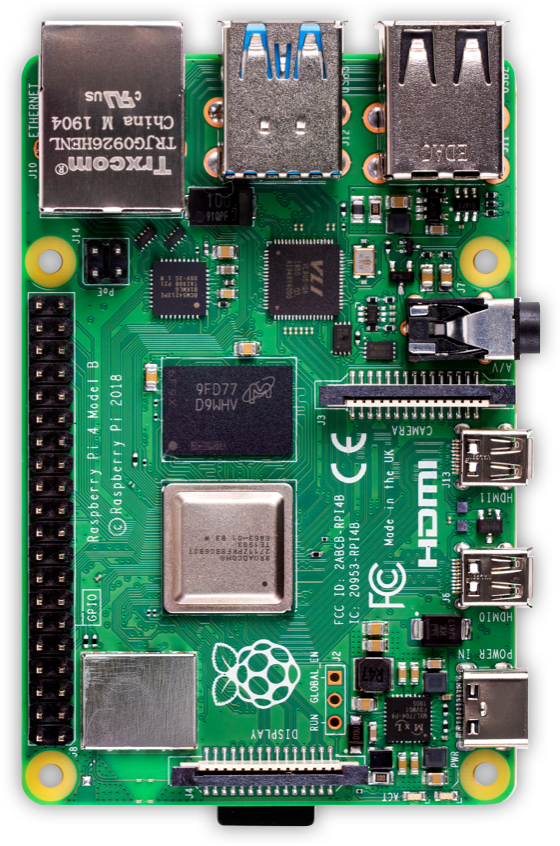
\includegraphics[width=0.85\linewidth]{images/components/raspberry-pi-4.png} 
\caption{Raspberry pi 4B}
\label{fig:wrapfig}
\end{wrapfigure}
Il Raspberry è un computer in miniatura sviluppato e prodotto dalla \textbf{Raspberry pi Foundation}. Si tratta di un computer a scheda singola dotato di un SoC ARM  prodotto da Broadcom.\\ 
In questo progetto abbiamo utilizzato la versione 4B, l'ultima rilasciata dalla casa produttrice e con le seguenti caratteristiche:
\begin{itemize}
    \item \textbf{CPU} -- Broadcom BCM2711, Quad core Cortex-A72 (ARM v8) 64-bit SoC 1.8GHz
    \item \textbf{RAM} -- 4 Gb DDR4
    \item \textbf{Interfacce video} -- 2x Micro HDMI ports
    \item \textbf{Interfacce USB} \begin{itemize}
        \item USB type C per alimentazione
        \item  2x USB 2.0
        \item  2x USB 3.0
    \end{itemize}
    \item \textbf{Interfacce di rete}\begin{itemize}
        \item Gigabit Ethernet
        \item  2.4 GHz e 5.0 GHz IEEE 802.11ac Wi-Fi
        \item  Bluetooth 5.0
    \end{itemize}
    \item \textbf{Dispositivi esterni} -- Supporto per camera e display MIPI
    \item \textbf{Interfacce GPIO} -- Header GPIO con 40 pin
\end{itemize}
\vspace{0.5cm}

\begin{wrapfigure}{r}{0.2\textwidth}
\vspace{-30pt}
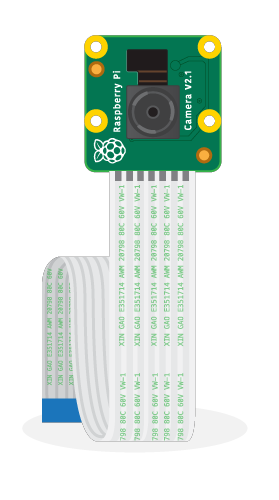
\includegraphics[width=0.9\linewidth]{images/components/pi-camera.png} 
\caption{Raspberry Pi Camera}
\label{fig:wrapfig}
\vspace{30pt}
\end{wrapfigure}
\subsection*{Camera Pi Module}

La Raspberry Pi Camera è un modulo che si collega direttamente alla porta CSI situata sul Raspberry.\\Questa, nella versione 1.3 utilizzata, consente di catturare immagini con risoluzione massima di 5 MPixel e video a 1080p 30 fps, nonostante il basso costo a cui viene venduta(intorno ai 15 Euro).\\
\vspace{0.5cm}

\subsection*{Arduino Nano}
\begin{wrapfigure}{r}{0.30\textwidth}
\vspace{20pt}
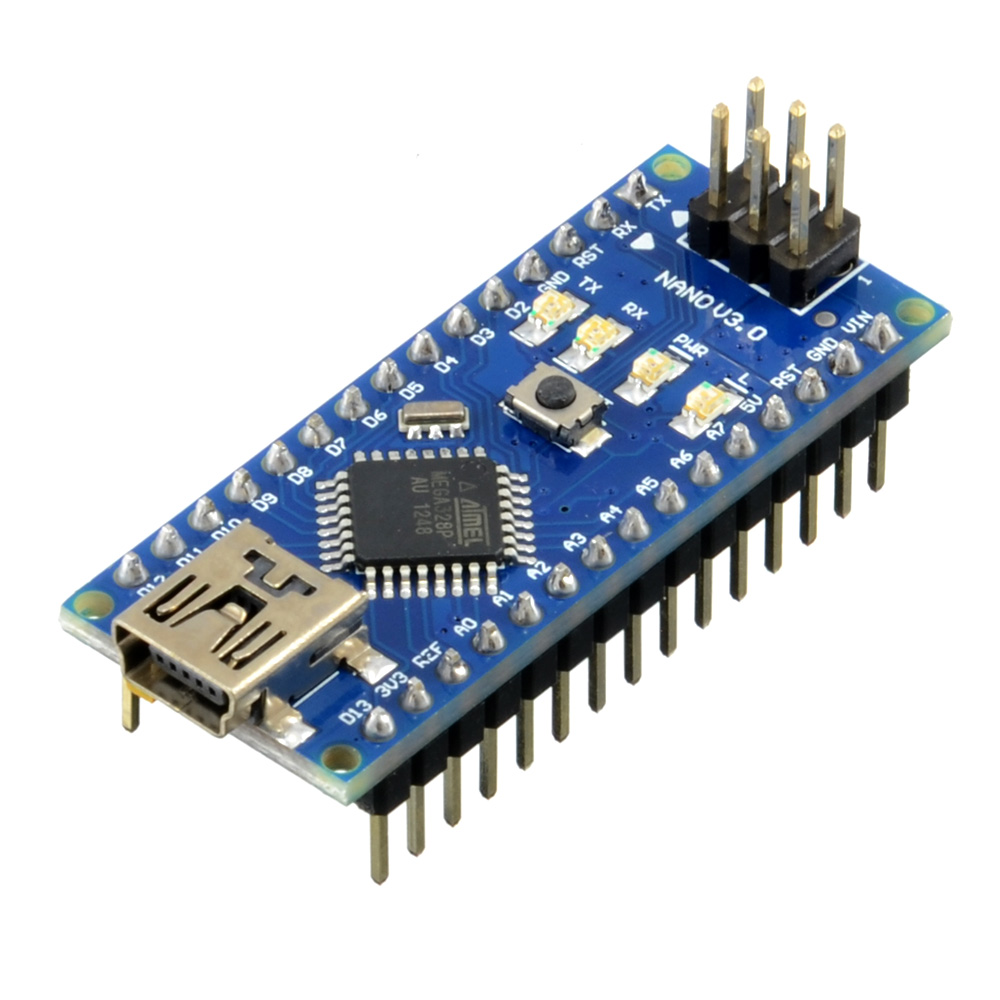
\includegraphics[width=0.85\linewidth]{images/components/arduino_nano.jpg} 
\caption{Arduino Nano v3}
\vspace{-20pt}
\label{fig:wrapfig}
\end{wrapfigure}
Arduino è un'azienda italiana specializzata nella produzione di micro-controllori, utilizzati soprattutto per piccoli progetti homemade o per didattica.\\
In questo progetto è stato utilizzato Arduino Nano v3, per le seguenti caratteristiche:

\begin{itemize}
    \item Dimensioni notevolmente ridotte, adatte anche al posizionamento su una breadboard
    \item Alimentazione a 5 Volt e comunicazione seriale via micro-usb 
    \item Dotato di micro-controllore ATmega328, lo stesso della versione più "potente" Arduino Uno 
    \item Presenza di 12 porte GPIO, anche con PWM (Pulse With Modulation) ed anche 6 porte per letture analogiche
\end{itemize}
\vspace{0.5cm}

\newpage
\subsection*{L298N DC Motor Controller}
\begin{wrapfigure}[8]{r}{0.25\textwidth}
\vspace{-40pt}
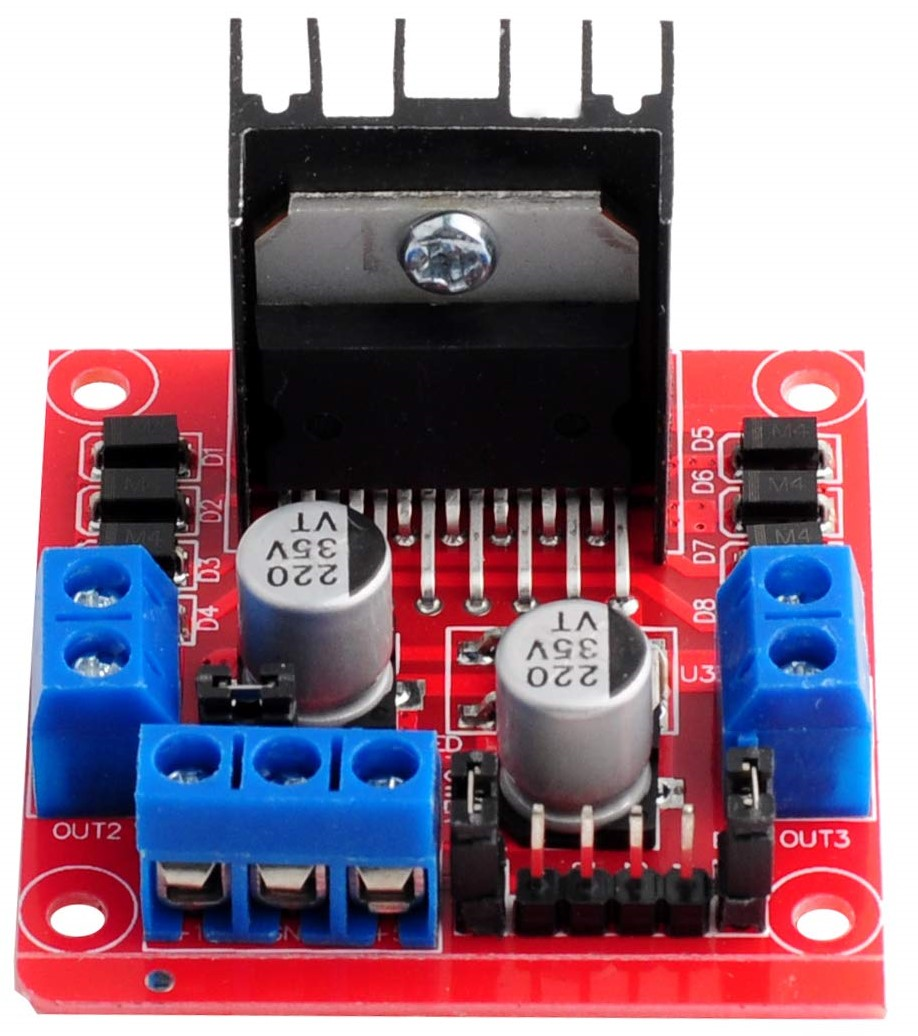
\includegraphics[width=0.9\linewidth]{images/components/l298n.jpg} 
\caption{L298N DC Motor Controller}
\vspace{+40pt}
\label{fig:wrapfig}
\end{wrapfigure}
Questo modulo, dotato di un chip L298N, consente di controllare due motori a spazzola (o corrente diretta) con un range operativo di 5- 35 Volt tramite dei segnali a 5 volt.\\
La velocità ed il verso di rotazione di entrambi i motori è controllabile tramite i pin situati nella parte frontale, insieme all'alimentazione; l'output dei motori si trova invece sui lati.\\



\begin{table}[h]
    \centering
    \rowcolors{2}{green!0!}{orange!10!}
    \begin{tabular}{ |c|p{7cm}|  }
    \hline
    \rowcolor{blue!35}\multicolumn{2}{|c|}{\Large\textbf{L298N Motor Controller Pinout}} \\
    \hline
    \textbf{VCC} & Alimentazione del modulo, range 7 - 24 Volt\\
    \textbf{GND} & Ground\\
    \textbf{+5V} & Output di 5V per alimentazione di controllori o periferiche esterne\\
    \hline
    \textbf{ENA} & Segnale PWM (0-255) per regolare la velocità del motore A\\
    \textbf{IN1 e IN2} & Impostano il verso del motore A\\
    \textbf{IN3 e IN4} & Impostano il verso del motore B\\
    \textbf{ENB} & Segnale PWM (0-255) per regolare la velocità del motore B\\
    \hline
    \end{tabular}
    \caption{L298N Motor Controller Pinout}
    \label{tab:requisiti_funzionali}
\end{table}
\vspace{0.5cm}


\subsection*{Motori a corrente diretta}
Per far muovere Stalker-Bot sono stati utilizzati 4 motori a corrente diretta (2 per lato) dotati di scatola con riduttore, questo aumenta la coppia del motore a scapito della velocità.
\FloatBarrier
\begin{figure}
\centering
    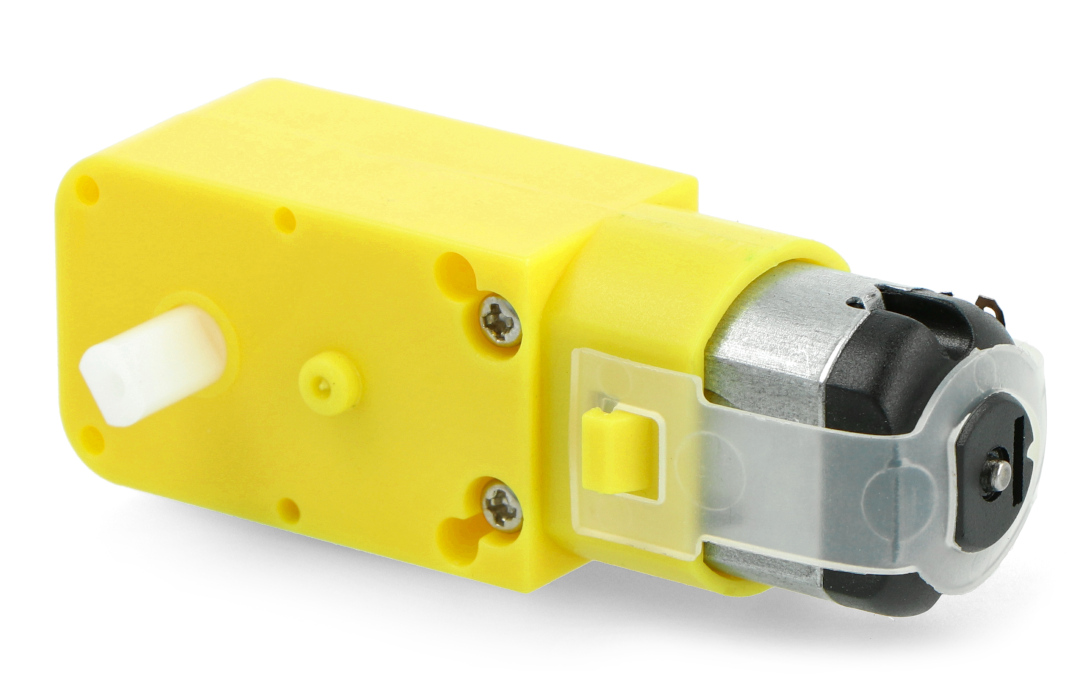
\includegraphics[width=0.25\linewidth]{images/components/motor_geared.jpg} 
    \caption{DC Motor with gearbox}
    \label{fig:wrapfig}
\end{figure}
\FloatBarrier


\subsection*{Batterie}
\begin{wrapfigure}[10]{r}{0.25\textwidth}
\centering
\vspace{-30pt}
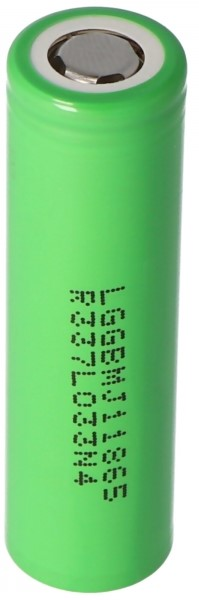
\includegraphics[width=0.4\linewidth]{images/components/18650.jpg} 
\caption{L298N DC Motor Controller}
\vspace{+30pt}
\end{wrapfigure}
L'alimentazione ai motori viene fornita da due batterie agli ioni di Litio, in particolare le 18650.\\ Esse sono batterie ricaricabili,hanno un range di voltaggio da 3.6 a 4.2 Volt e una buona autonomia (circa 5000 mAh ognuna); inoltre l'output massimo di corrente di 4 A consente di avere sufficiente alimentazione per il movimento di un robot cingolato.\\
Vengono utilizzate due batterie alla volta, posizionate in serie in modo da ottenere un voltaggio finale che varia da 7.4 a 8.4 Volt.


\subsection*{Powerbank e cablaggi}

Per l'alimentazione del Raspberry pi sarà necessario utilizzare un powerbank che riesca a fornire almeno 15 Watt di potenza.\\
Per quanto riguarda i cablaggi, saranno necessari due cavetti usb, uno per collegare il powerbank al Raspberry e l'altro il Raspberry all'Arduino Nano. Oltre a questo serviranno dei cavetti jumper ed una breadboard, per collegare Arduino alle periferiche.

\begin{figure}[!h]
    \centering
    \begin{minipage}{.5\textwidth}
        \centering
        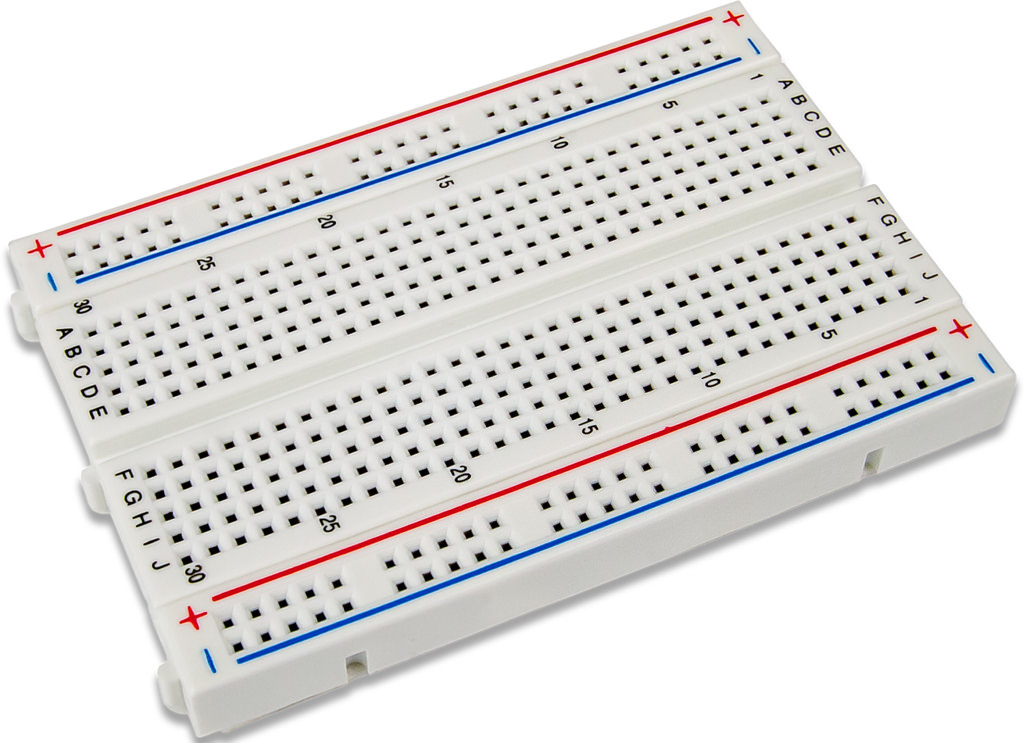
\includegraphics[width=0.85\linewidth, height=0.18\textheight]{images/components/breadboard.jpg}
        \caption{Breadboard}
    \end{minipage}%
    \begin{minipage}{0.5\textwidth}
        \centering
        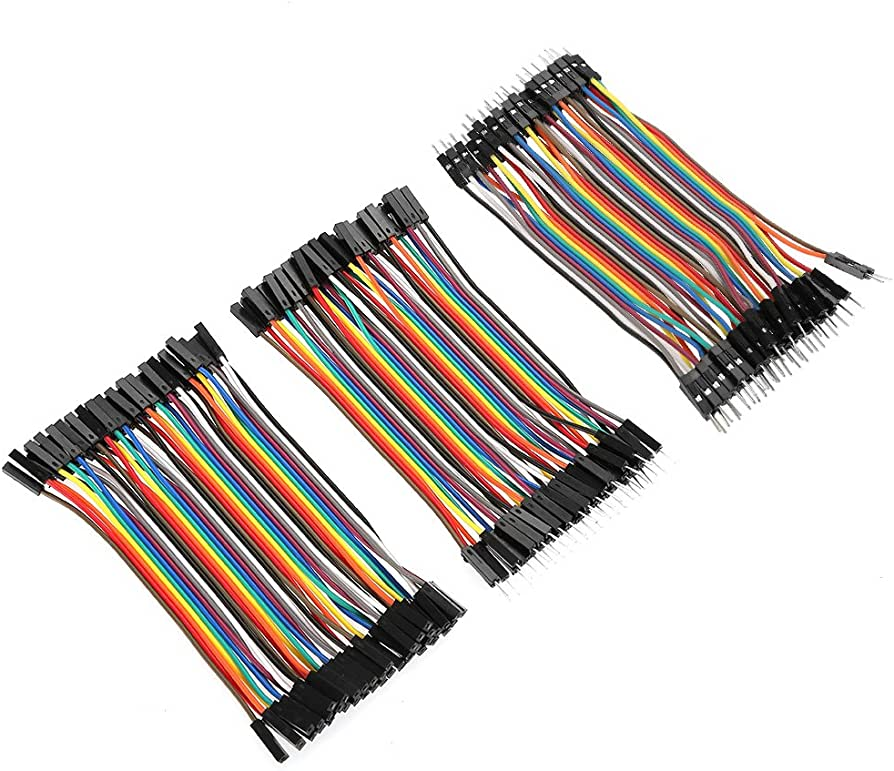
\includegraphics[width=0.65\linewidth, height=0.18\textheight]{images/components/jumpers.jpg}
        \caption{Jumper wires}
    \end{minipage}
\end{figure}


\newpage
\section{Collegamenti}

Di seguito viene riportato lo schema dei collegamenti fra Arduino Nano e le periferiche di Stalker-Bot.

\FloatBarrier
\begin{figure}[!h]
    \centering
    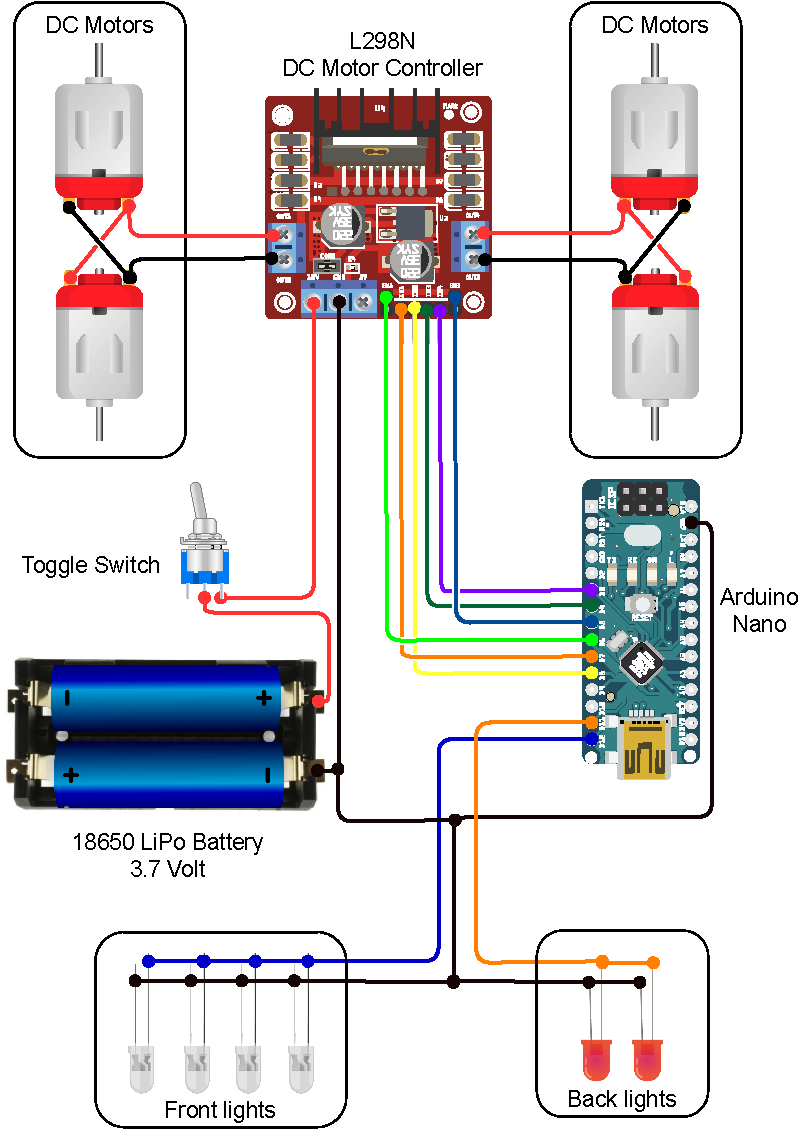
\includegraphics[width=12cm]{images/circuito.drawio.pdf}
    \caption{Wiring Stalker-Bot}
\end{figure}
\FloatBarrier

La comunicazione fra il Raspberry ed Arduino avviene invece tramite comunicazione seriale via USB.

\FloatBarrier
\begin{figure}[!h]
    \centering
    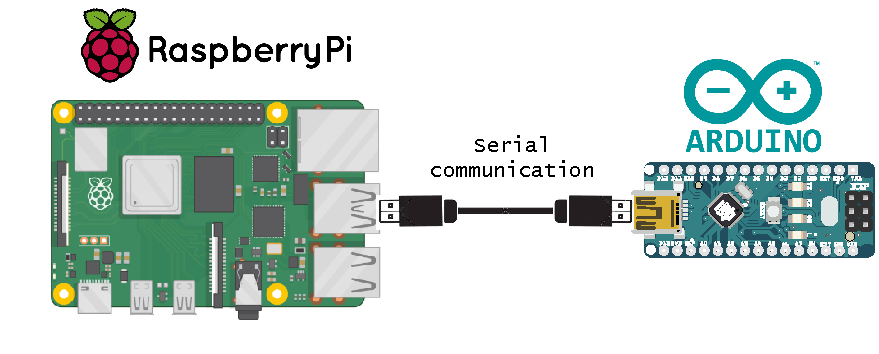
\includegraphics[width=10cm]{images/raspberry-arduino.pdf}
    \caption{Comunicazione seriale}
\end{figure}
\FloatBarrier

\section{Scocca}

\subsection{Modellazione 3D}

La scocca di Stalker-Bot è stata progettata utilizzando Autodesk Fusion 360. I modelli ed i file STL (per la stampa) sono reperibili reperibili sul sito thingiverse\footnote{Modelli: https://www.thingiverse.com/thing:6069512}.

\FloatBarrier
\begin{figure}[!ht]
    \centering
    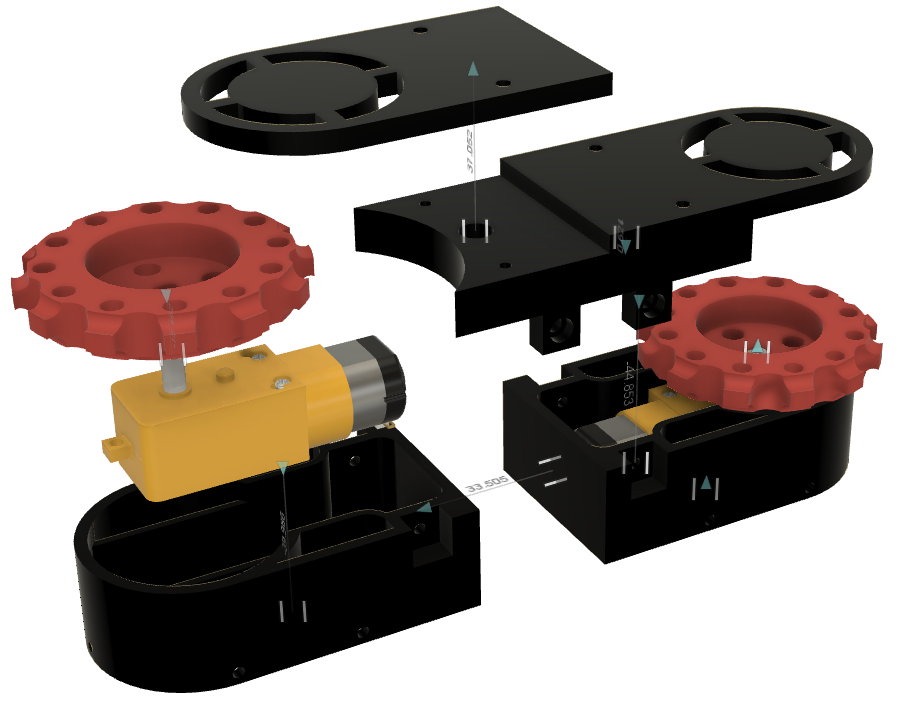
\includegraphics[width=13cm]{images/motori_no_spigoli.png}
    \caption{Assieme motore}
\end{figure}
\FloatBarrier

\FloatBarrier
\begin{figure}[!ht]
\begin{adjustwidth}{-2cm}{}
    \centering
    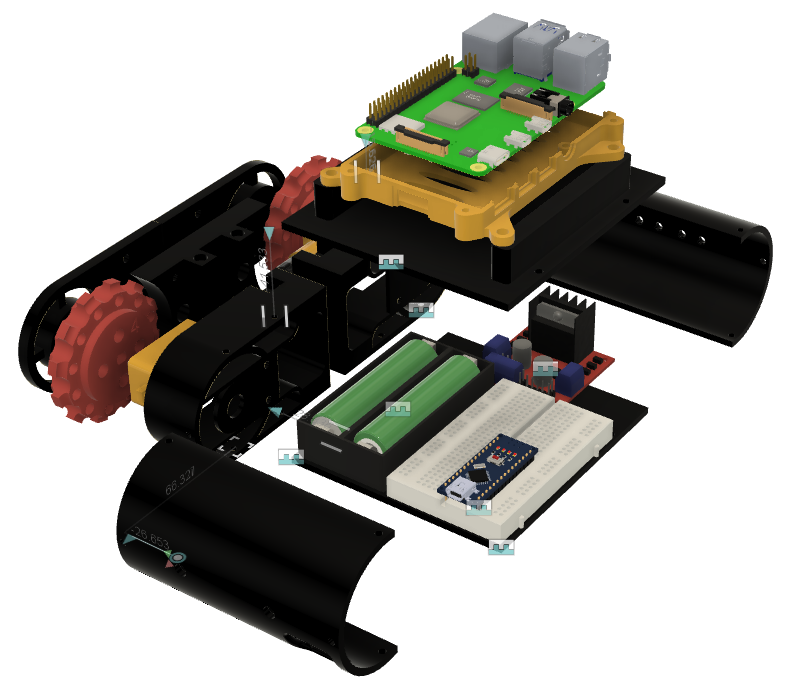
\includegraphics[width=18cm]{images/assieme_stalker_bot.png}
    \caption{Assieme Stalker-Bot}
\end{adjustwidth}
\end{figure}
\FloatBarrier

\subsection{Stampa 3D}
\begin{wrapfigure}[10]{r}{0.25\textwidth}
\centering
\vspace{-50pt}
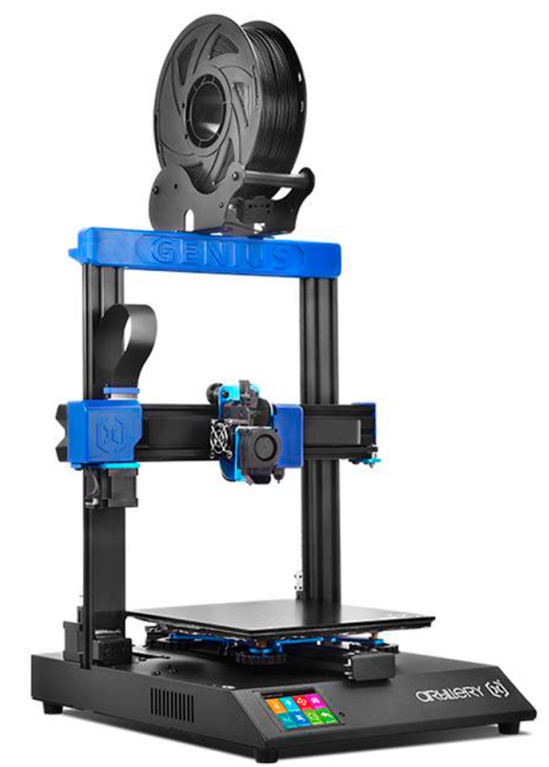
\includegraphics[width=0.9\linewidth]{images/components/stampante.png} 
\caption{Stampante 3D}
\vspace{+50pt}
\end{wrapfigure}
L'intera scocca dello Stalker-Bot è stata stampata in 3D, compresi i cingoli. È stata utilizzata la stampante fdm Artillery Genius.\\
I materiali utilizzati sono PETG rosso e nero (scocca ed ingranaggi) e PLA giallo (cingoli e case Raspberrry).

\subsection{Assemblaggio}
Per l'assemblaggio saranno necessari due "assieme motore", cioè la parte in cui vengono situati i motori insieme agli ingranaggi che poi metteranno in moto i cingoli.\\
I due "blocchi motore" vengono quindi collegati dal case del robot, all'interno del quale si trovano Arduino, il controller dei motori e le batterie.\\
Sopra la scocca vengono montati quindi il powerbank, il Raspberry e la Pi Camera.

\subsection{Risultato}

\FloatBarrier
\begin{figure}[!h]
    \centering
    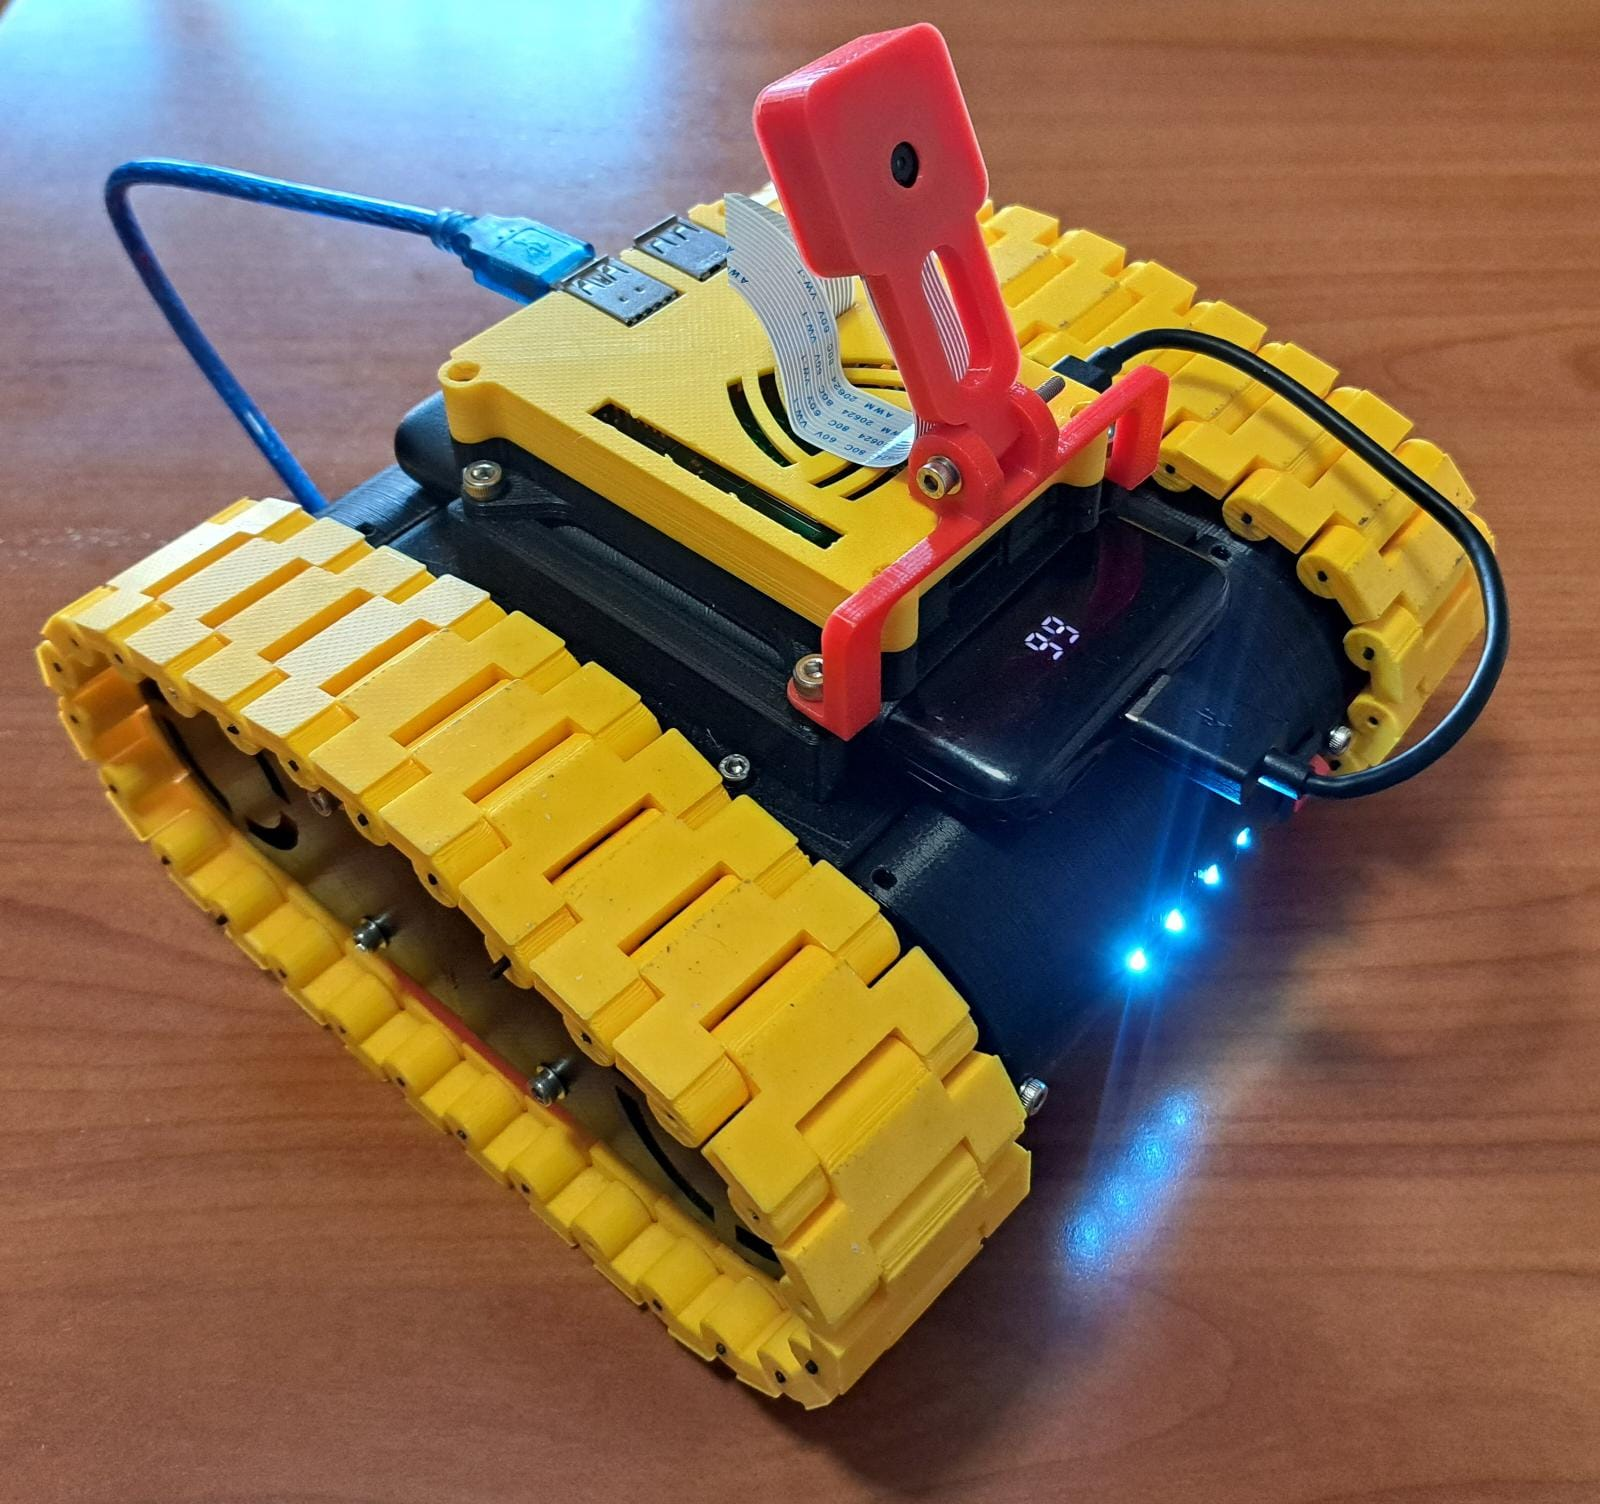
\includegraphics[width=13cm]{images/robot-front.jpg}
    \caption{Stalker-Bot fronte}
\end{figure}

\begin{figure}[!h]
    \centering
    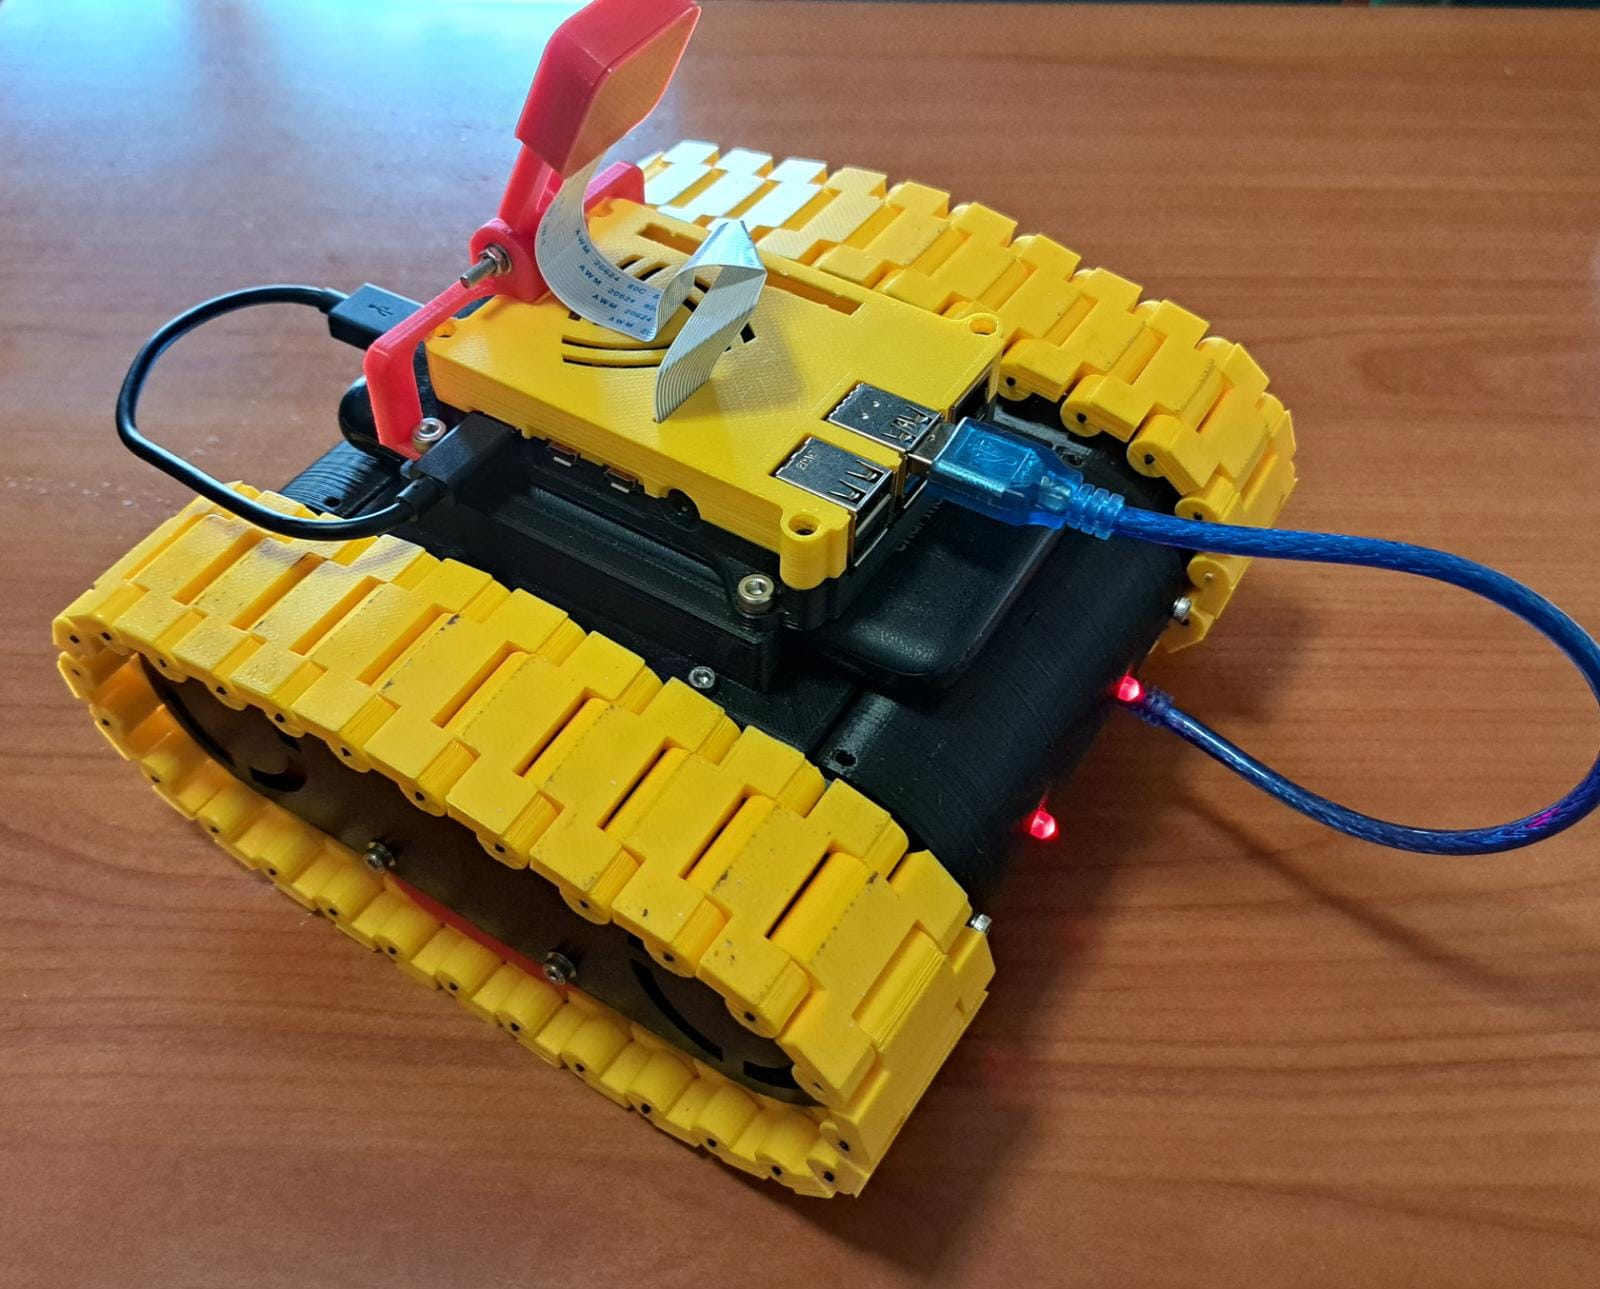
\includegraphics[width=11cm]{images/robot-back.jpg}
    \caption{Stalker-Bot retro}
\end{figure}

\begin{figure}[!h]
    \centering
    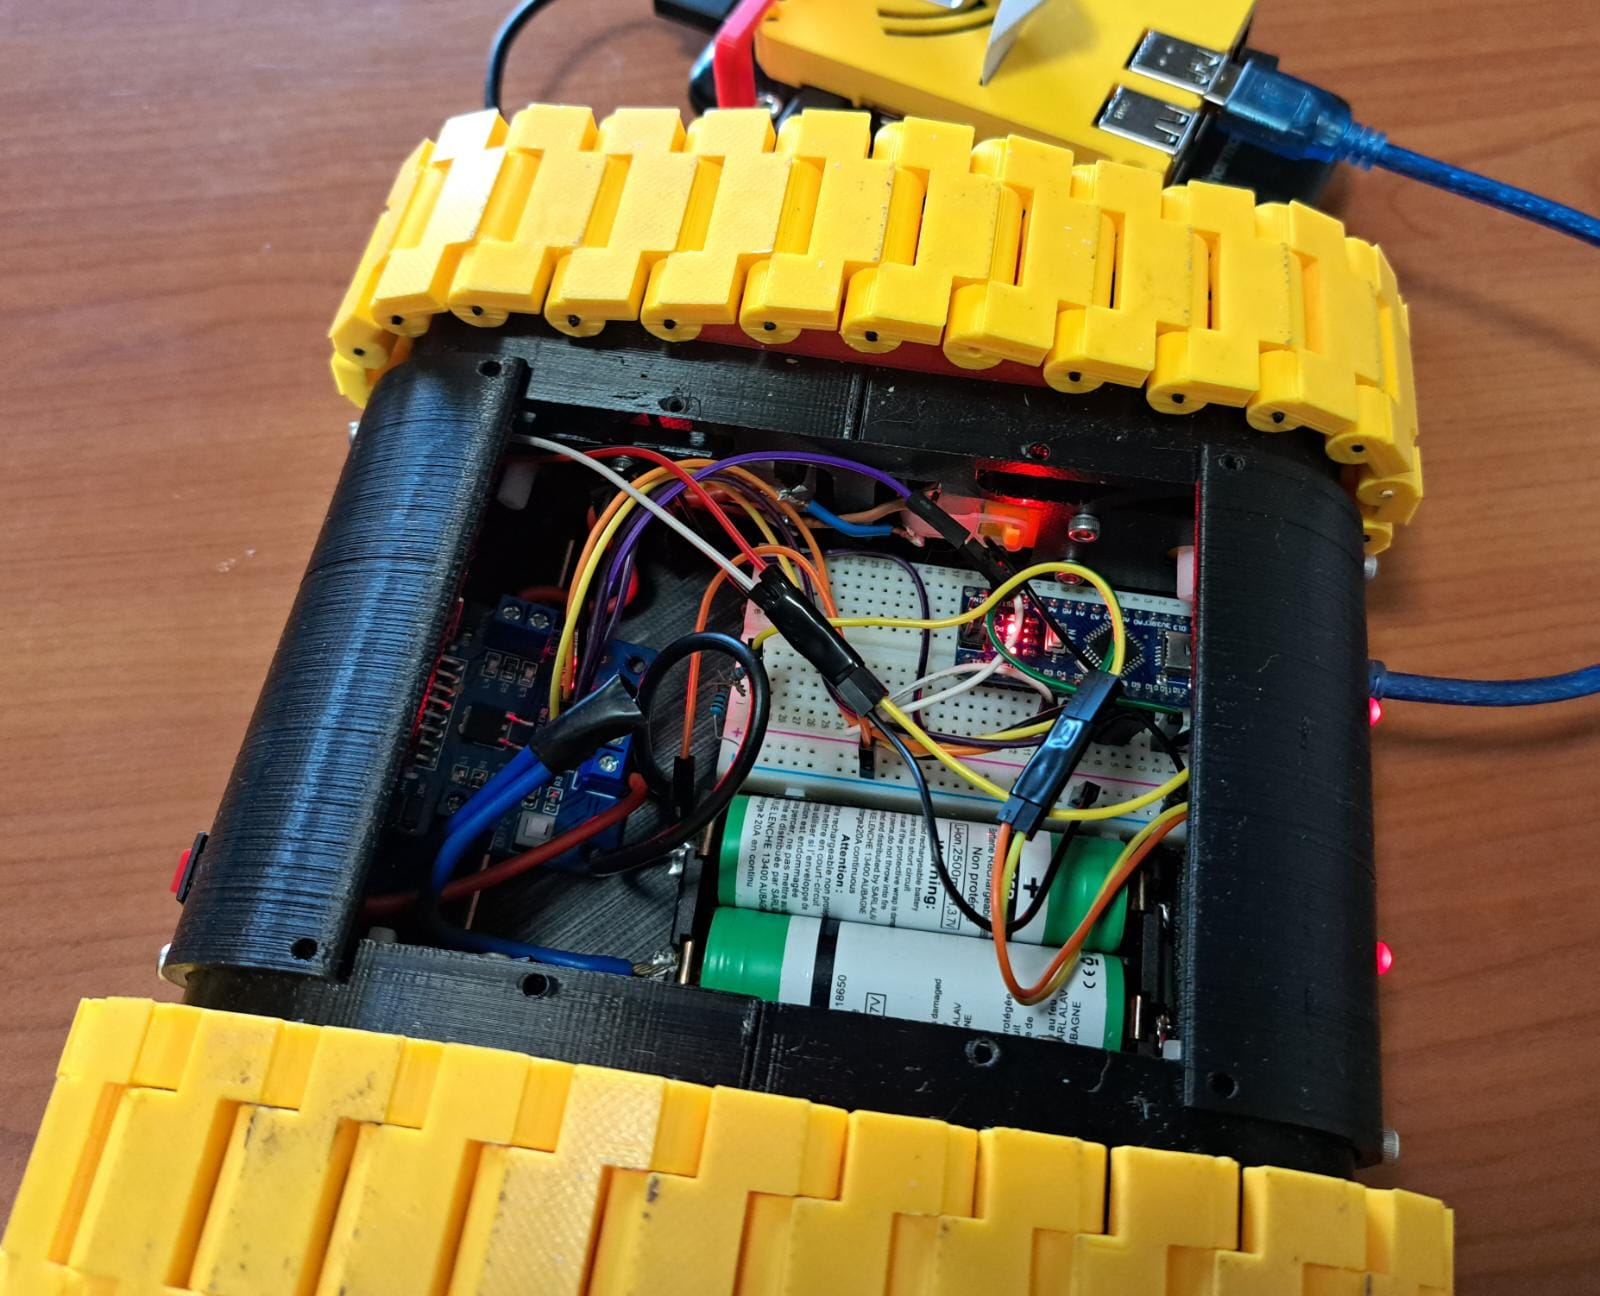
\includegraphics[width=11cm]{images/robot-cablaggi.jpg}
    \caption{Stalker-Bot cablaggi}
\end{figure}
\FloatBarrier



\chapter{Implementazione}
\label{cap: Implementazione}
Per la fase di addestramento prima e di riconoscimento facciale dopo, \`e stato impiegato un classificatore di volti umani preaddestrato, offerto da OpenCV in formato XML.
In particolare, il modello utilizzato "haarcascade\_frontalface\_default.xml"   \`e in grado di identificare volti umani all'interno di un frame.
Nelle prossime sezioni non viene riportato il codice per intero, che rimane comunque consultabile all'indirizzzo $\\$\href{https://github.com/Lore09/Stalker-bot}{"https://github.com/Lore09/Stalker-bot"}, ma solo le parti ritenute fondamentali. 

\section{Addestramento}
La fase di addestramento si divide in due ulteriori fasi: una prima in cui vengono catturati trenta frame al proprietario e una seconda in cui viene effettivamente addestrato il riconoscitore.$\\$
\subsection{Cattura immagini del proprietario}
Acquisizione camera:
\begin{minted}
[
framesep=2mm,
baselinestretch=1,
bgcolor=uclablue!14!!,
fontsize=\small,
breaklines
]{python}
cam = cv2.VideoCapture(0)
cam.set(3, 640)  # set video width
cam.set(4, 480)  # set video height
\end{minted}
Inizializzazione del riconoscitore tramite il modello preaddestrato:
\begin{minted}
[
framesep=2mm,
baselinestretch=1,
bgcolor=uclablue!14!!,
fontsize=\small,
breaklines
]{python}
cascadePath = "classifier/haarcascade_frontalface_default.xml"
detector = cv2.CascadeClassifier(cascadePath)
\end{minted}
Acquisizione di un frame dalla camera, conversione del frame in scala di grigi per rendere computazionalmente pi\`u leggera l'identificazione dei volti:
\begin{minted}
[
framesep=2mm,
baselinestretch=1,
bgcolor=uclablue!14!!,
fontsize=\small,
breaklines
]{python}
ret, img = cam.read()
gray = cv2.cvtColor(img, cv2.COLOR_BGR2GRAY)
faces = detector.detectMultiScale(gray, 1.3, 5)
\end{minted}
Ciascun volto localizzato viene racchiuso in un rettangolo e quest'ultimo viene codificato in quattro valori, rispettivamente: coordinata iniziale lungo l'asse orizzontale (x), coordinata iniziale lungo l'asse verticale (y), larghezza (w) e altezza (h).
Per ogni volto riconosciuto viene salvata un'immagine in formato .jpg che ha dimensioni pari a quelle del rettangolo che racchiude il volto stesso:
\begin{minted}
[
framesep=2mm,
baselinestretch=1,
bgcolor=uclablue!14!!,
fontsize=\small,
breaklines
]{python}
for (x, y, w, h) in faces:
    cv2.imwrite("dataset/User." + str(face_id) + '.' + str(count) + ".jpg", gray[y:y + h, x:x + w])
\end{minted}
\subsection{Addestramento del riconoscitore}
Come riconoscitore viene istanziata una classe, sempre fornita da OpenCV, che verr\`a successivamente allenata per riconoscere i volti precedentemente salvati:
\begin{minted}
[
framesep=2mm,
baselinestretch=1,
bgcolor=uclablue!14!!,
fontsize=\small,
breaklines
]{python}
recognizer = cv2.face.LBPHFaceRecognizer_create()
\end{minted}
Viene definito il metodo getImagesAndLabels(path) (qui non riportato) che restituisce: le immagini dal dataset sotto forma di numpy array e il nome dell'utente associato a quelle immagini. Successivamente viene allenato il riconoscitore e viene salvato il modello appena creato:
\begin{minted}
[
framesep=2mm,
baselinestretch=1,
bgcolor=uclablue!14!!,
fontsize=\small,
breaklines
]{python}
path = 'dataset'

faces,ids = getImagesAndLabels(path)
recognizer.train(faces, np.array(ids))

# Save the model into trainer/trainer.yml
recognizer.write( path + '/trainer.yml')
\end{minted}

\section{Esecuzione Stalker-Bot}

Una volta addestrato il riconoscitore è possibile mettere in moto Stalker-Bot.\\ Il software in questo caso viene eseguito sia su Raspberry (riconoscimento e generazione comandi) che su Arduino (conversione comandi del raspberry in comandi per i motori).

\subsection{Riconoscimento}
In questa sezione viene mostrato come effettivamente \`e possibile utilizzare il riconoscitore (allenato nella sezione precedente) affinch\'e riconosca il suo padrone in un flusso video.
Inizialmente viene effettuato un setup in cui: viene inizializzato il riconoscitore (LBPHFaceRecognizer\_create()), quest'ultimo legge il modello creato durante la fase di addestramento, viene inizializzato un detector, con lo stesso classificatore preaddestrato visto nell'introduzione del capitolo \ref{cap: Implementazione}, che si occuper\`a di cercare, all'interno di ciascun frame, dei volti umani. Viene, inoltre, riportata l'acquisizione della camera:
\begin{minted}
[
framesep=2mm,
baselinestretch=1,
bgcolor=uclablue!14!!,
fontsize=\small,
breaklines
]{python}
recognizer = cv2.face.LBPHFaceRecognizer_create()
recognizer.read('dataset/trainer.yml')
cascadePath = "classifier/haarcascade_frontalface_default.xml"
faceCascade = cv2.CascadeClassifier(cascadePath);

# Initialize and start realtime video capture
cam = cv2.VideoCapture(0)
cam.set(3, 640)  # set video widht
cam.set(4, 480)  # set video height
\end{minted}
A ciascun frame (prima convertito in scala di grigi per alleggerire il carico computazionale) viene applicata la normalizzazione per ottenere un contrasto maggiore. Quindi si cercano, al loro interno, i volti:
\begin{minted}
[
framesep=2mm,
baselinestretch=1,
bgcolor=uclablue!14!!,
fontsize=\small,
breaklines
]{python}
ret, img = cam.read()

gray = cv2.cvtColor(img, cv2.COLOR_BGR2GRAY)
    
normalised_image = np.zeros((300, 300))
imageNp = cv2.normalize(gray, normalised_image, 0, 255, cv2.NORM_MINMAX)

faces = faceCascade.detectMultiScale(
            imageNp,
            scaleFactor=1.2,
            minNeighbors=5,
            minSize=(int(minW), int(minH))
        )
\end{minted}
Ogni volto umano localizzato viene passato al riconoscitore che restituisce l'identificatore di ciascuno dei volti presenti nel dataset usato per l'addestramento con associato un valore (confidence) che rappresenta quanto il volto localizzato si avvicina al volto presente nel dataset: 
\begin{minted}
[
framesep=2mm,
baselinestretch=1,
bgcolor=uclablue!14!!,
fontsize=\small,
breaklines
]{python}
for (x, y, w, h) in faces:
    id, confidence = recognizer.predict(imageNp[y:y + h, x:x + w])
\end{minted}


\subsection{Movimento}
Una volta riconosciuto il proprietario, Stalker-bot deve seguire i movimenti del suo volto. Per fare ciò lo script calcola quanto la faccia del proprietario si discosta dal centro dell'immagine, entro un certo range.\\
Viene inoltre definita la funzione \verb|arduino_map()|, utile per convertire valori appartenenti a domini differenti.
\begin{minted}
[
framesep=2mm,
baselinestretch=1,
bgcolor=uclablue!14!!,
fontsize=\small,
breaklines
]{python}
x_delta = 50
y_delta = 45

def arduino_map(value, in_min, in_max, out_min, out_max):
    return (value - in_min) * (out_max - out_min) / (in_max - in_min) + out_min    
\end{minted}

Il seguente algoritmo prende le coordinate x ed y corrispondenti alla faccia del proprietario e li utilizza per calcolare i valori di sterzata ed accelerazione del robot.
\begin{minted}
[
framesep=2mm,
baselinestretch=1,
bgcolor=uclablue!14!!,
fontsize=\small,
breaklines
]{C++}
mid_x = x + w / 2
mid_y = y + h / 2
  
turn = 0
acc = 0

if mid_x < (640 / 2 - x_delta) or mid_x > (640 / 2 + x_delta):
    turn = int(arduino_map((mid_x - (640 / 2 + x_delta)), -640/2 + x_delta, 640/2 - x_delta, -75, 75))

if mid_y < (480 / 2 - y_delta) or mid_y > (480 / 2 + y_delta):
    acc = int(arduino_map((mid_y - (480 / 2 + y_delta)), -480/2 + 
    y_delta, 480/2 - y_delta, -75, 75))
\end{minted}

Questi valori vengono poi utilizzati per comporre il comando che verrà inviato, tramite comunicazione seriale, ad Arduino.\\
La struttura del comando è \verb|acceleration,turn,time\n| in cui time è la durata del comando (in millisecondi), acceleration e turn rispettivamente la velocità di avanzamento e di sterzata e variano nel range (-100,100).

\begin{minted}
[
framesep=2mm,
baselinestretch=1,
bgcolor=uclablue!14!!,
fontsize=\small,
breaklines
]{python}
    string = str(acc) + "," + str(turn) + ",100\n"
    ser.write(string.encode('utf-8'))    
\end{minted}

\subsection{Arduino}

Di seguito viene riportato il codice in esecuzione su Arduino Nano. Questo script si occupa di leggere i dati in arrivo dalla comunicazione seriale con il Raspberry, impartire i comandi ai motori e alle luci.\\
All'inizio vengono inizializzate le variabili globali:
\begin{minted}
[
framesep=2mm,
baselinestretch=1,
bgcolor=uclablue!14!!,
fontsize=\small,
breaklines
]{C++}
// Motor A connections
int enA = 6;
int in1 = 7;
int in2 = 8;
// Motor B connections
int enB = 5;
int in3 = 4;
int in4 = 3;

// Lights
int front_led = 12;
int back_led = 11;

// Motor control variables
int base_pwm = 100;  // Base PWM value to sent to motors (Range 0-255), adjust to match your motors
int turn_speed = 0; // Target value for turning (Range -255 to 255)
int advance_speed = 0; // Target value for advancing (Range -255 to 255)
int leftMotorSpeed = 0;  // PWM value for left motor (Range 0 to 255)
int rightMotorSpeed = 0; // PWM value for right motor (Range 0 to 255)
long command_start_time = 0; // Time of last command
long command_duration = 0; // Duration of last command
\end{minted}

La funzione moveMotors() si occupa di convertire i valori acceleration e turn in arrivo dal Raspberry in comandi per i due motori.
\begin{minted}
[
framesep=2mm,
baselinestretch=1,
bgcolor=uclablue!14!!,
fontsize=\small,
breaklines
]{C++}
void moveMotors(int advanceSpeed, int turnSpeed){

    rightMotorSpeed = advanceSpeed + turnSpeed;
    leftMotorSpeed = advanceSpeed - turnSpeed;

    if(leftMotorSpeed == 0 && rightMotorSpeed == 0) {
      stop();
      return;
    }
    if(leftMotorSpeed > 0) {
        analogWrite(enA, leftMotorSpeed + base_pwm);   
        digitalWrite(in1, HIGH);
        digitalWrite(in2, LOW);
    } else{
        analogWrite(enA, -(leftMotorSpeed - base_pwm));
        digitalWrite(in1, LOW);
        digitalWrite(in2, HIGH);
    }
    if(rightMotorSpeed > 0){
        analogWrite(enB, rightMotorSpeed + base_pwm);
        digitalWrite(in3, HIGH);
        digitalWrite(in4, LOW);
    } else {
        analogWrite(enB, -(rightMotorSpeed - base_pwm));
        digitalWrite(in3, LOW);
        digitalWrite(in4, HIGH);
    }
}
\end{minted}

La funzione stop() viene utilizzata per fermare tutti i motori ed impostare le velocità a 0.
\begin{minted}
[
framesep=2mm,
baselinestretch=1,
bgcolor=uclablue!14!!,
fontsize=\small,
breaklines
]{C++}
void stop(){
  digitalWrite(in1, LOW);
  digitalWrite(in2, LOW);
  digitalWrite(in3, LOW);
  digitalWrite(in4, LOW);
  analogWrite(enA, 0);
  analogWrite(enB, 0);
}
\end{minted}

La funzione checkPortaSeriale() si occupa di controllare se nella coda della comunicazione seriale sono presenti dei comandi e, nel caso ci siano, di ottenerne i valori.
\begin{minted}
[
framesep=2mm,
baselinestretch=1,
bgcolor=uclablue!14!!,
fontsize=\small,
breaklines
]{C++}
bool checkSerialData(){
  if (Serial.available() > 0) {
    String data = Serial.readStringUntil('\n');
    // Direct commands
    switch (data[0])
    {
    case 'F': // Front lights 
      if(data.substring(2).toInt() == 1){
        digitalWrite(front_led, HIGH);
      } else {
        digitalWrite(front_led, LOW);
      }
      break;
    case 'B': // Back lights
      if(data.substring(2).toInt() == 1){
        digitalWrite(back_led, HIGH);
      } else {
        digitalWrite(back_led, LOW);
      }
      break;
    case 'S': // Emergency stop
      stop();
      turn_speed=0;
      advance_speed=0;
      break;
    default: // movement command
      // split value,value,value by comma
      int firstComma = data.indexOf(',');
      int secondComma = data.indexOf(',', firstComma + 1);
      // get advance, turn and command duration
      advance_speed = data.substring(0, firstComma).toInt();
      turn_speed = data.substring(firstComma + 1, secondComma).toInt();
      command_duration = data.substring(secondComma + 1).toInt();
      break;
    }
    return true;
  }
  else return false;
}
\end{minted}

All'interno della funzione Setup(), che verrà eseugita una sola volta all'avvio del programma, vengono impostati i GPIO in modalità OUTPUT e viene avviata la comunicazione seriale, con baud rate 9600.
\begin{minted}
[
framesep=2mm,
baselinestretch=1,
bgcolor=uclablue!14!!,
fontsize=\small,
breaklines
]{C++}
void setup() {
// Set all the motor control pins to outputs
pinMode(enA, OUTPUT);
pinMode(enB, OUTPUT);
pinMode(in1, OUTPUT);
pinMode(in2, OUTPUT);
pinMode(in3, OUTPUT);
pinMode(in4, OUTPUT);
pinMode(front_led, OUTPUT);
pinMode(back_led, OUTPUT);

// Begin serial communication at a baudrate of 9600:
Serial.begin(9600);
delay(1000);
}
\end{minted}

La funzione loop() è quella che viene eseguita a regime. Ad ogni iterazione il programma controlla la porta seriale e, se sono presenti nuovi comandi, resetta lo \verb|start_time| del comando.\\
A questo punto, se la durata del comando in esecuzione è inferiore a quella massima specificata nel comando stesso, il programma muoverà i motori utilizzando i valori specificati; in caso la durata superi quella massima il robot verrà fermato.

\begin{minted}
[
framesep=2mm,
baselinestretch=1,
bgcolor=uclablue!14!!,
fontsize=\small,
breaklines
]{C++}

void loop() {
    if(checkSerialData()){
        command_start_time = millis(); // Reset starting time
    };
  // Move motors
  if(millis() - command_start_time < command_duration){
    moveMotors(advance_speed, turn_speed);
  }
  else {
    stop();
    Serial.println("STOP");
  }
  delay(10);
}
\end{minted}




\chapter*{Conclusioni}
\addcontentsline{toc}{chapter}{Conclusioni}
Questo progetto si \`e concentrato sull'integrazione tra sistemi embedded, machine learning e computer vision, in particolare sullo sviluppo di un robot in grado di individuare la posizione di un volto, verificare che questo coincida con quello del suo proprietario e di seguirne i movimenti.
Si è visto come \`e possibile addestrare, con una serie di immagini, una rete affinch\'e possa riconoscere, durante un flusso video, un volto umano.
Un eventuale sviluppo futuro di questo progetto potrebbe essere
quello di sostituire la Picamera con una camera a pi\`u alta risoluzione, in modo da poter incrementare il grado di confidenza durante la fase di riconoscimento facciale.

%%%%%%%%%% BIBLIOGRAPHY %%%%%%%%%%%%%%
\cleardoublepage
\nocite{*}
\printbibliography[title=Sitografia]
\addcontentsline{toc}{chapter}{Sitografia}



\end{document}